\section*{Introduction}

%\begin{frame}
%	\frametitle{Visibility Control}
%	\only<1>{This text is only on slide 1.}
%	\uncover<2-3>{This text is uncovered on slides 2 and 3.}
%	\visible<2>{This text becomes visible on slide 2.}
%	\invisible<3>{This text becomes invisible on slide 3.}
%\end{frame}

\begin{frame}{Introduction}
	\only<1>{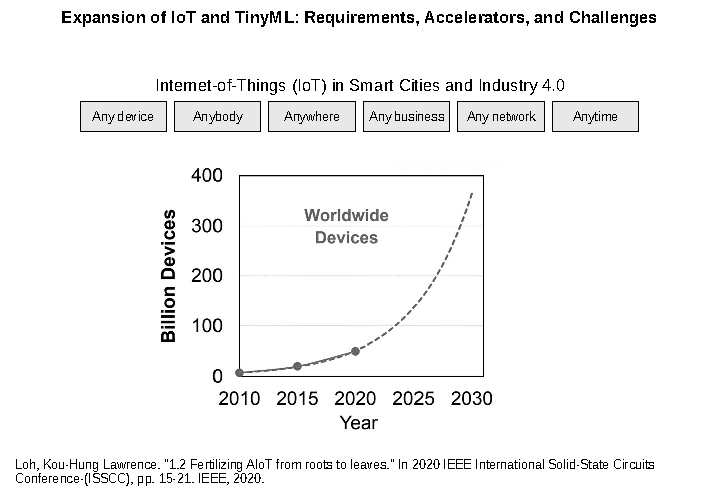
\includegraphics[width=\textwidth]{slides/Introduction/1.pdf}}
	\only<2>{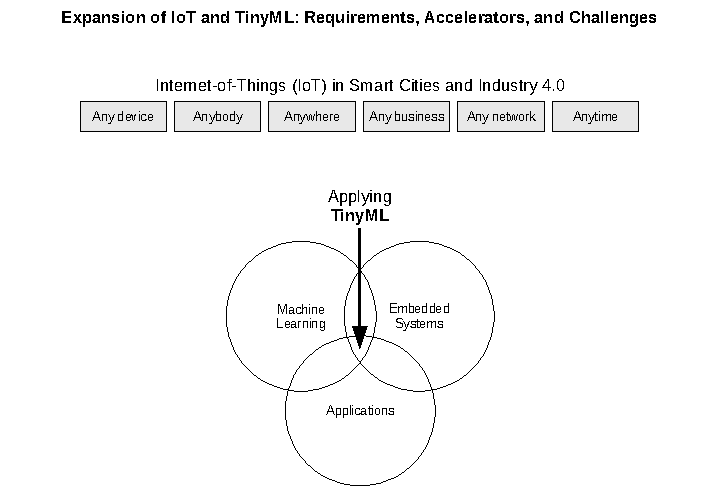
\includegraphics[width=\textwidth]{slides/Introduction/2.pdf}}
	\only<3>{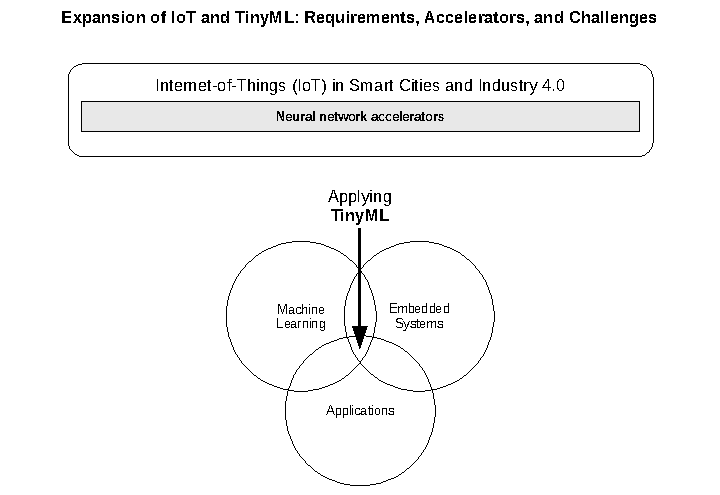
\includegraphics[width=\textwidth]{slides/Introduction/3.pdf}}
	\only<4>{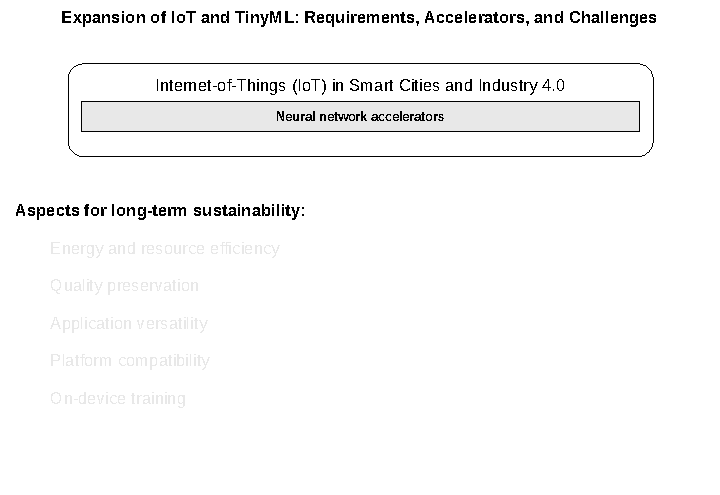
\includegraphics[width=\textwidth]{slides/Introduction/4.pdf}}
	\only<5>{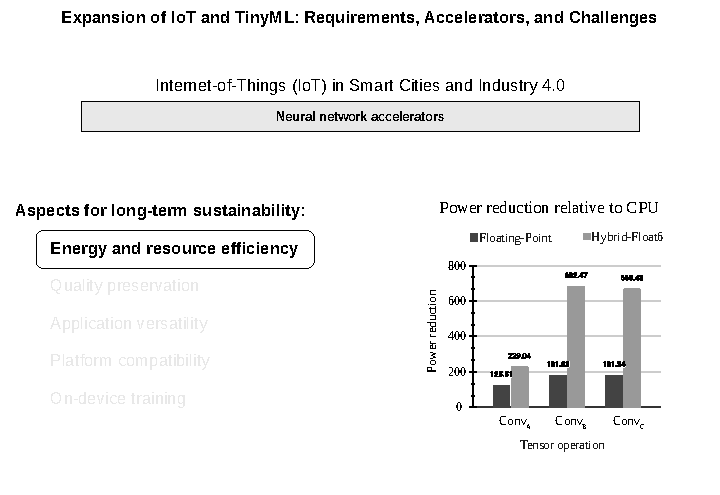
\includegraphics[width=\textwidth]{slides/Introduction/5.pdf}}
	\only<6>{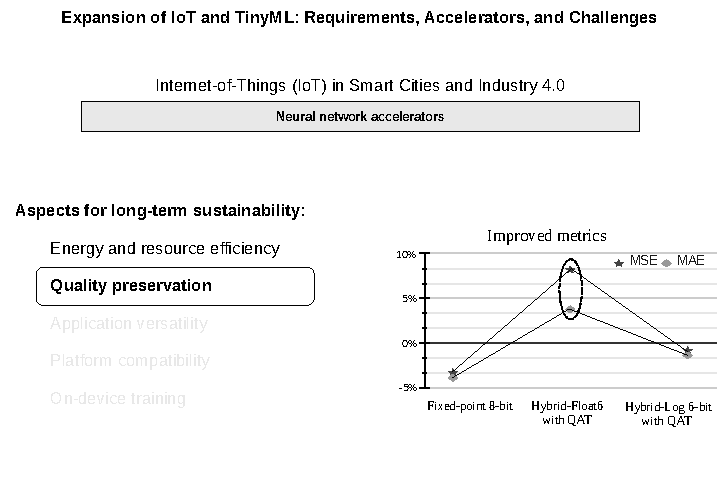
\includegraphics[width=\textwidth]{slides/Introduction/6.pdf}}
	\only<7>{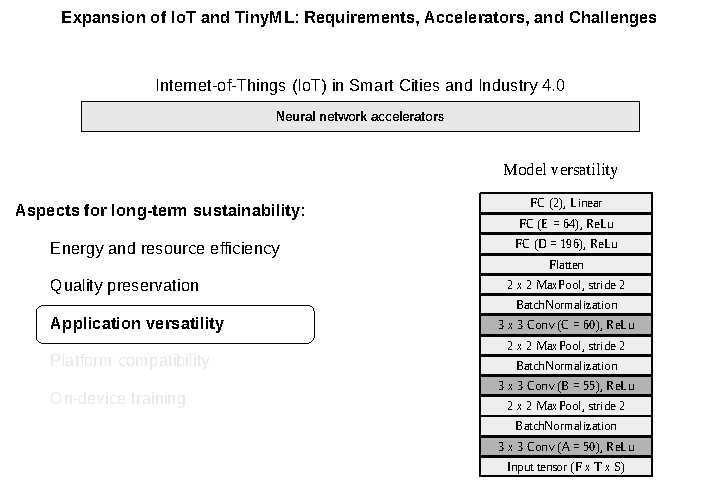
\includegraphics[width=\textwidth]{slides/Introduction/7.pdf}}
	\only<8>{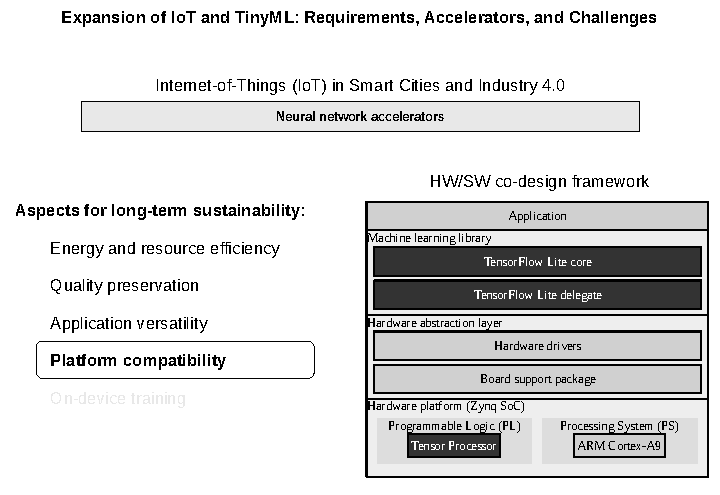
\includegraphics[width=\textwidth]{slides/Introduction/8.pdf}}
	\only<9>{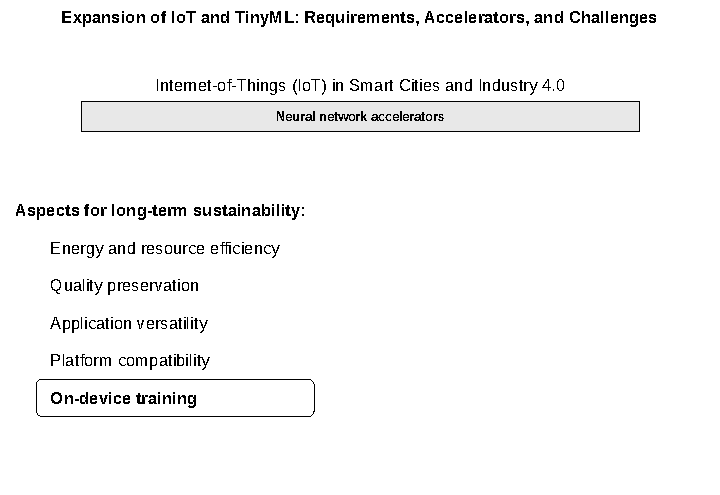
\includegraphics[width=\textwidth]{slides/Introduction/9.pdf}}
	\only<10>{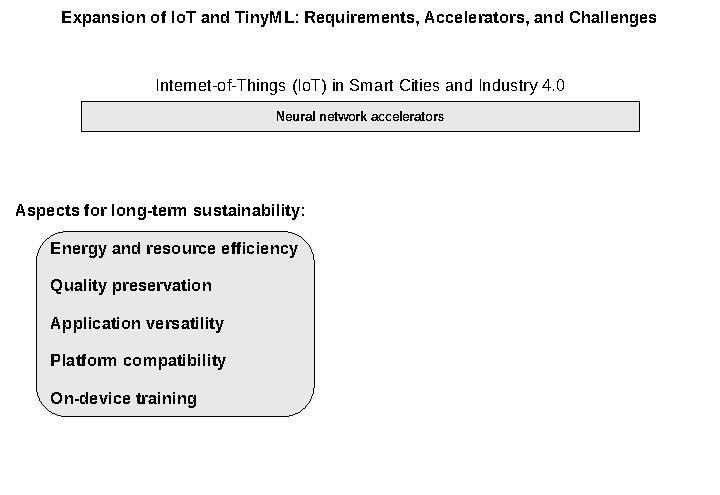
\includegraphics[width=\textwidth]{slides/Introduction/10.pdf}}
	\only<11>{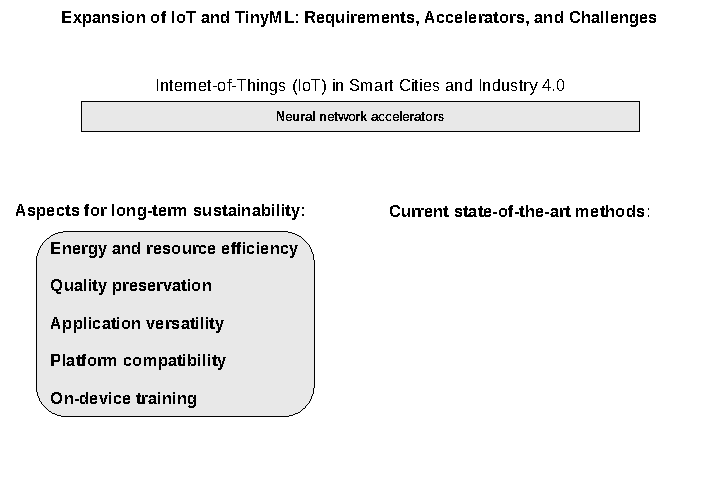
\includegraphics[width=\textwidth]{slides/Introduction/11.pdf}}
	\only<12>{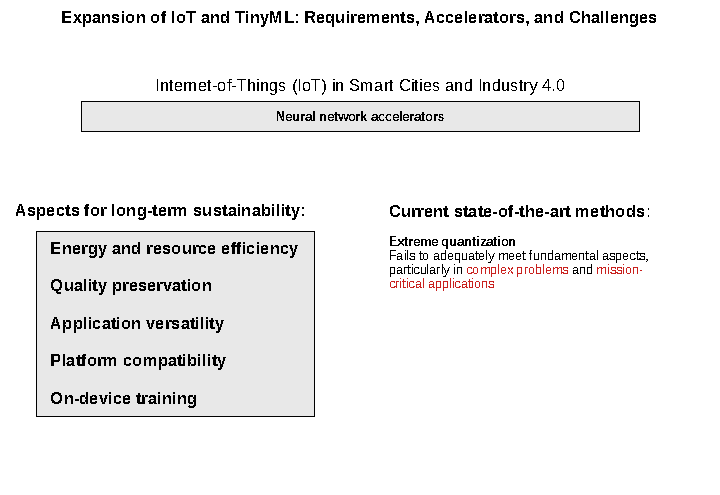
\includegraphics[width=\textwidth]{slides/Introduction/12.pdf}}
	\only<13>{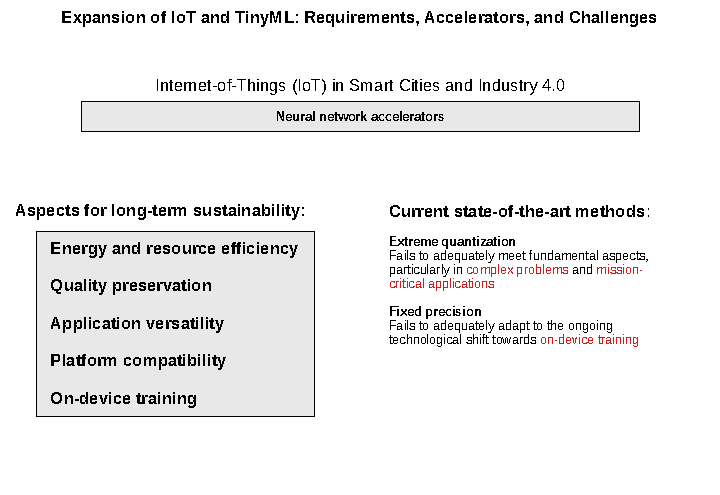
\includegraphics[width=\textwidth]{slides/Introduction/13.pdf}}
\end{frame}
	
	\section*{Goal and Objectives}
	\begin{frame}
		\frametitle{Goal and Objectives}
		\begin{itemize}
			\item<1-> \textbf{Goal}:
			To establish a sustainable, efficient, and universally applicable neural network acceleration technique that supports inference and facilitates on-device training in extreme edge devices, ensuring future-proof and broad applicability. This approach integrates hybrid custom floating-point (FP) computation.
			
			\vspace{10mm} 
			
			\item<2-> \textbf{Objectives}:
			\begin{itemize}
				\item<3-> Investigate custom FP computation
				\item<4-> Conduct performance evaluation
				\item<5-> Analyze impact
				\item<6-> Ensure cross-platform compatibility
			\end{itemize}
		\end{itemize}
	\end{frame}

	\begin{frame}
	\frametitle{Outline}
	\tableofcontents % This command automatically creates a table of contents based on the sections and subsections
	\end{frame}